\subsection{Einstieg und Wiederhohlung}

\subsubsection{$\sin$ und $\cos$ im rechtwinkligem Dreieck}
Der $\sin$ ist das Verhältnis von der Gegenkathete zur Hypothenuse im rechtwinkligem Dreieck.\\~ \\
$\frac{Gegenkathete}{Hypothenuse}=\sin(\alpha)=\cos(\beta)$\\~\\
Der $\cos$ ist das Verhältnis der Ankathete im Vergleich zur Hypothenuse im rechtwinkligem Dreieck

\subsubsection{$\sin$ \& $\cos$ im Kreis}
\paragraph*{$\sin$ am Einheitskreis}~\\
Die Welle ist das Verhältnis des Sinus am Einheitskreis auf eine x-Achse übertragen.
\paragraph*{$\cos$ am Einheitskreis}~\\
Die Welle ist das Verhältnis des Cosinus am Einheitskreis auf eine x-Achse übertragen.\\~\\
\hyperlink{https://upload.wikimedia.org/wikipedia/commons/f/f3/Sinus_und_Cosinus_am_Einheitskreis.gif}{\textcolor{RedViolet}{\textbf{\fcolorbox{red}{white}{Darstellung von $\sin$ und $\cos$ im Einheitskreis}}}}\\
\input{Sem1/MINT/Mathe_Lasowski/Tabelle_Bogenmaß}
\subsubsection{Additionstheoreme}
\begin{center}
    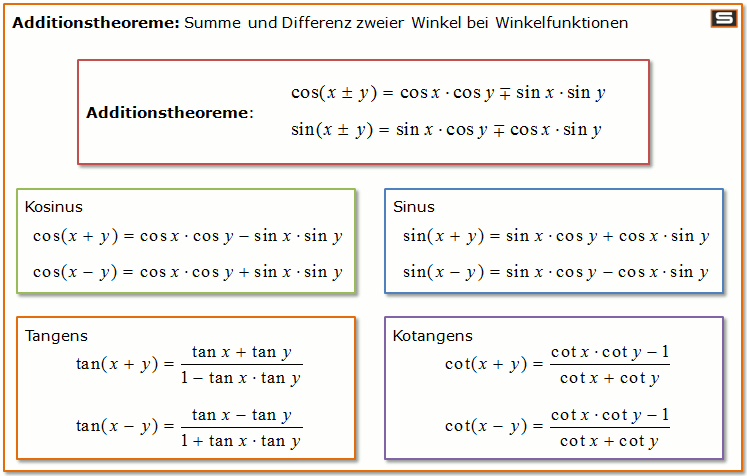
\includegraphics[width=1\textwidth]{Sem1/MINT/Bilder/Additionstheoreme_Trigonometrie.png}
\end{center}
$sin(x+y)=sin(x)*cos(y)+cos(x)*sin(y)$\\
$sin(30+120)=sin(30)*cos(120)+cos(30)*sin(120)$\\
$=\frac12*-\frac12+\frac{\sqrt3}{2}*\frac{\sqrt3}{2}$\\
$=-\frac14+\frac34=\underline{\frac12}$
\paragraph*{allgemeiner Fall}~\\
\begin{center}
    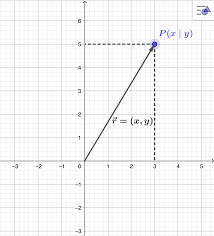
\includegraphics[width=100px]{Sem1/MINT/Bilder/download 1.png}
\end{center}
